\documentclass{Preport}

\usepackage{placeins}
\usepackage{hyperref}
\usepackage{amsmath}
\hypersetup{
    colorlinks=true,
}

\exname{非平衡电桥} %实验名称
\instructor{谭艾林} %指导教师
\class{github} %班级
\name{MJ} %姓名
\stuid{2025} %学号

\nyear{2025} %年
\nmonth{12} %月
\nday{29} %日
\nweekday{一} %星期几

\begin{document}
\setcounter{page}{0}
\makecover

\section{预习报告（10分）}
\subsection{实验综述（5分）}

平衡电桥一般用于测量相对稳定的物理量，要测量连续变化的电桥需要采用非平衡电桥。
实际上是相应传感器元件受到特定的外界环境变化而引起内阻变化，通过非平衡电桥将阻值转化为电压输出，
达到测量和控制环境变化的目的。

如图为非平衡电桥的结构：

\begin{figure}[htpb!]
    \centering
    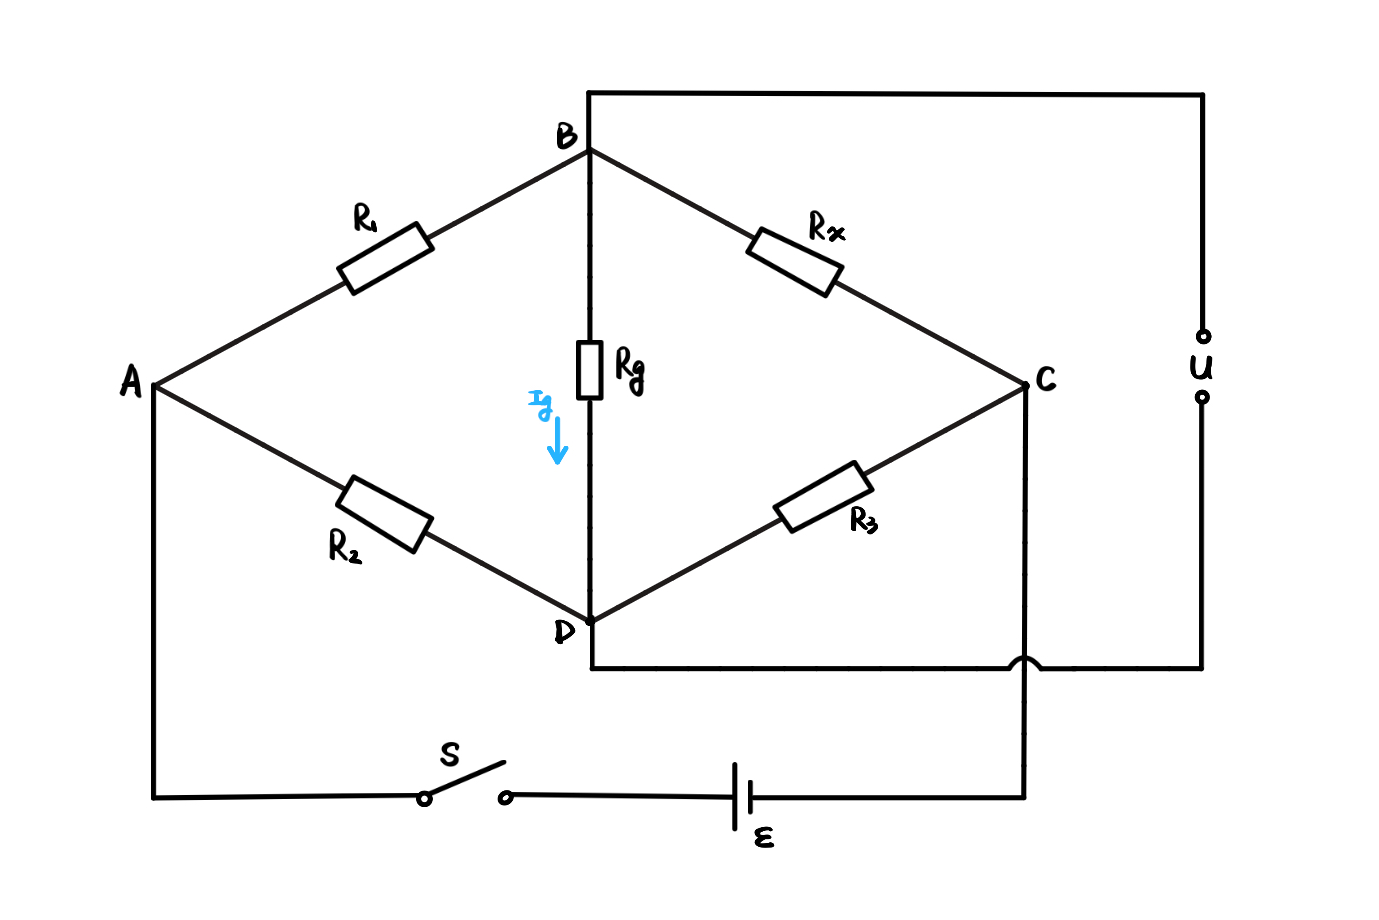
\includegraphics[width=0.5\textwidth]{demo.PNG}
\end{figure}

当负载电阻 $R_g \to \infty$ 时，有 $I_g = 0$ ，输出电压为

\[
U = U_{BC} - U_{DC} = \frac{R_2 R_x - R_1 R_3}{(R_1 + R_x)(R_2 + R_3)} \epsilon
\]

当满足 $R_1 R_3 = R_2 R_x$ 时，易知电桥输出电压为零，处于平衡状态；
而如果固定 $R_1 、 R_2 、 R_3$ ，待测电阻 $R_x$ 变为 $R_x + \Delta R_x$ 后，
电桥会因不平衡而产生输出电压：

\[
U = \frac{R_2 R_x + R_2 \Delta R_x - R_1 R_3}{(R_1 + R_x + \Delta R_x)(R_2 + R_3)} \epsilon
\]

测量这个输出电压，就可以求出电阻 $R_x$ 的变化值 $\Delta R_x$ 。

测量变温金属的电阻温度系数时，由于处于室温且温度变化不大，金属阻值随温度近似呈线性关系：

\[
R_t = R_0 (1 + \alpha t)
\]

其中 $t$ 为摄氏温度， $R_0$ 是 $t = 0 ℃$ 的阻值， $\alpha$ 是电阻温度系数。

调节至 $R_1 = R_2 = R_3 = R_0$ 与 $R_x = R_t$ ，代入输出非平衡电压，化简后有:

\[
\alpha = \frac{4 U}{t (\epsilon - 2 U)}
\]

\subsection{实验重点（3分）}

本实验的重点在于掌握非平衡直流电桥的工作原理和测量方法，并能够应用非平衡直流电桥测量金属材料
的温阻特性和电阻温度系数。

\subsection{实验难点（2分）}

本实验的难点主要在于要精确调节非平衡电桥的起始平衡状态，考虑电桥灵敏度；
在金属电阻温度变化的过程中控制速度，使得阻值与温度读数准确对应；以及减小接触电阻等干扰。

$\quad$

\input{注意事项}
\end{document}
